Objasnićemo apstraktnu interpretaciju na primeru \emph{propagacije konstanti}. 
Cilj nam je da otkrijemo u svakoj tački funkcije da li bilo koja od promenljivih koja se koristi u toj tački ima konstantnu vrednost, tj. da li ima istu vrednost nezavisno od ulaznih parametara funkcije i nezavisno od toga koji deo koda je izvršen u toj funkciji. 
Prevodioci koriste ovaj tip analize za optimizaciju propagacije konstanti, što znači menjanje konstantnih promenljivih kontantama. 
Ovo je primer C++ koda koji ćemo analizirati, sa komentarima koji ukazuju na konstantne promenljive.
\lstinputlisting[language=C++, caption=Primer koda]{snippets/ex1.cpp}

\subsection{Grafovi kontrole toka}
\label{subsec:cfgs}

\begin{figure}
\begin{center}
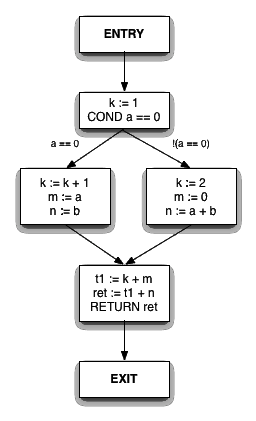
\includegraphics[scale=0.5]{Treehydra-cfg.png}
\end{center}
\caption{Primer grafa kontole toka}
\label{fig:graf}
\end{figure}

Apstraktna interpretacija se obavlja nad dijagramom koji predstavlja funkciju koju ispitujemo, i zove se \emph{graf kontrole toka (eng. control flow graph, CFG}). Na slici \ref{fig:graf} je prikazan graf funkcije koju ćemo ispitivati. \\
Neke napomene:
\begin{itemize}
\item Svi mogući prelazi su prikazani kao ivice, tj. veze između čvorova koji sadrže kod
\item Naredbe imaju tačno jednu operaciju i najviše jednu dodelu. Privermene promenljive se dodaju po potrebi.
\end{itemize}

Terminologija:
\begin{itemize}
\item Svaki čvor se zove \textbf{osnovni blok} \emph{(eng. basic block, \textbf{BB})}. Osnovni blok se definiše tako što ima samo jednu tačku ulaza, i jednu tačku izlaza, što će reći da nema grananja unutar osnovnih blokova.
\item Naredbe ćemo zvati \emph{instrukcije}, iako one uopšteno mogu imati različite nazive u zavisnosti od toga koliko operanada primaju.
\item \textbf{Tačka u programu} je zamišljena tačka pre ili posle svake instrukcije. Funkcija ima dobro definisano stanje u svakoj tački, tako da će se naša analiza programa uvek referisati na ove tačke.
\end{itemize}


\subsection{Konkretna interpretacija}
\label{subsec:concreteimpr}
Kako bismo objasnili apstraktnu interpretaciju, počećemo prvo sa primerom konkretne interpretacije.
Kasnije ćemo se nadograditi na ovaj primer kako bismo objasnili apstraktnu interpretaciju. \\
Mogli bismo početi tako što bismo zvali funkciju za različite ulaze, i potom gledali koje su sve promenljive konstantne
kroz sve te pozive. Počnimo tako što ćemo pokrenuti program za ulaze \texttt{a=0, b=7}:
\verbatiminput{snippets/ex2_1.txt}
Dakle, \texttt{k = 2} pre nego što se koristi u naredbi \texttt{t1 := k + m}. Možemo pokrenuti funkciju za ostale ulaze i dobili bismo isti rezultat.
Međutim, ovakav način testiranja nam ne može potvrditi da je \texttt{k = 2} za sve moguće ulaze. (Doduše može, ali samo ako bismo proverili za svaki od $2^{64}$ ulaza.)


\subsection{Približavanje apstraktnoj interpretaciji}
\label{subsec:approachingabsint}
Ako pogledamo prethodnu funkciju, možemo primetiti da postoje samo dva bitna slučaja: \texttt{a == 0}, \texttt{a != 0}, dok
\texttt{b} nije bitno. 
Pokrenimo dva testa: jedan sa ulazom \texttt{a = 0, b = ?}, a drugi sa ulazom \texttt{a = NN, b = ?}, gde \textbf{NN} odznačava ne-nula vrednost, dok \textbf{?} označava bilo koju vrednost. Počnimo sa \texttt{a = 0, b = ?}:
\verbatiminput{snippets/ex2_2.txt}
Ovo izgleda poprilično isto kao i konkretan primer, samo što su sada neke vrednosti apstrahovane, \texttt{NN} i \texttt{?},
koje predstavljaju skupove konkretnih vrednosti.\\
Takođe moramo da znamo šta opeatori rade nad apstraktnim vrednostima. Na primer, u poslednjem koraku,
\texttt{ret := t1 + n} postaje \texttt{ret := 2 + ?}. Kako bismo saznali šta ovo znači, posmatramo skupove konkretnih vrednosti: Ako \texttt{?} može biti bilo koja vrednost, onda i \texttt{2 + ?} takođe može uzeti bilo koju vrednost, tako da \texttt{2 + ? -> ?}.
Preostali slučaj testira \texttt{a = NN, b = ?}:
\verbatiminput{snippets/ex2_3.txt}
Sada smo testirali za svaki mogući ulaz, kao i svaku granu koda funkcije. Ovo je dokaz da \texttt{k = 2} je uvek tačno
pre nego dođemo do \texttt{t1 := k + m}.\\
Procedura koju smo upravo ispratili daje određen uvid kako bismo bismo krenuli u proces apstraktne interpretacije, ali
nismo generalizovali samu proceduru. Tačno smo zali koje apstraktne vrednosti da koristimo za test slučajeve, i to smo mogli
samo zato što smo imali kao primer jednostavnu funkciju. Ova metoda neće biti primenjiva na komplikovane funckije, i nije
automatizovana.\\
Drugi problem je što smo posmatrali svaku granu funkcije posebno. Funckija sa \texttt{k} iskaza može imati i do
\texttt{$2^k$} grana, dok funkcija sa petljama ih može imati i beskonačno, i ovo nam onemogućava da imamo kompletnu
pokrivenost.

\subsection{Apstraktna interpretacija kroz primer}
\label{subsec:absintex}
Jedan od problema sa gornjim pristupom apstraktnoj interpretaciji je bio što nismo znali kako da odaberemo skupove
apstraktnih vrednosti koje ćemo koristiti kao ulaz za test primere. Pokušajmo da sprovedemo jedan test gde nećemo birati
takve skupove, dakle pokušajmo sa sledećim ulazom: \texttt{a = ?, b = ?}:
\verbatiminput{snippets/ex2_4.txt}
Šta sada? Nemamo informaciju o tome šta je \texttt{a}, tako da ne znamo kojom granom treba da idemo. Odabraćemo obe. 
Prvo za potvrdnu granu:
\verbatiminput{snippets/ex2_5.txt}
Potom za negativni slučaj:
\verbatiminput{snippets/ex2_6.txt}
U ovoj tački, dva izvršna toka se spajaju. Mogli bismo da nastavimo da ih testiramo ponaosob, ali znamo da će to dovesti
do eksplozije u uopštenom slučaju, tako da ćemo izvršiti spajanje stanja. Potrebno nam je jedno stanje koje pokriva obe
grane:
\verbatiminput{snippets/ex2_7.txt}
Ovo stanje možemo dobiti tako što ćemo spajati promenljivu po promenljivu. Na primer, \texttt{k} je 2 u jednom i u drugom
stanju, tako da je \texttt{k = 2} u rezultujućem stanju. Za \texttt{m}, ono može biti bilo šta u prvom stanju, tako da iako
je ono 0 u drugom stanju, može uzeti bilo koju vrednost u rezultujućem stanju. Kao rezultat dobijamo:  
\verbatiminput{snippets/ex2_8.txt}
Možemo nastaviti izvršavanje u jednom toku:
\verbatiminput{snippets/ex2_9.txt}
Gde dobijamo odgovor koji smo želeli, \texttt{k = 2}. Osnovne ideje su bile:
\begin{itemize}
\item Proći kroz funkciju koristeći apstraktne vrednosti kao ulaz
\item Apstraktna vrednost predstavlja skup konkretnih vrednosti
\item Kod kontrole toka gde imamo grananje, krenimo put obe grane
\item Gde imamo spajanje, spajamo izlaz iz obe grane
\end{itemize}
\cite{MozWiki}

